\documentclass[12pt, titlepage]{article}

\usepackage{booktabs}
\usepackage{changepage}
\usepackage{tabularx}
\usepackage{hyperref}
\usepackage{adjustbox}

\hypersetup{
    colorlinks,
    citecolor=blue,
    filecolor=black,
    linkcolor=red,
    urlcolor=blue
}
\usepackage[round]{natbib}
\usepackage{float}
\usepackage{graphicx}

%% Comments

\usepackage{color}

\newif\ifcomments\commentstrue %displays comments
%\newif\ifcomments\commentsfalse %so that comments do not display

\ifcomments
\newcommand{\authornote}[3]{\textcolor{#1}{[#3 ---#2]}}
\newcommand{\todo}[1]{\textcolor{red}{[TODO: #1]}}
\else
\newcommand{\authornote}[3]{}
\newcommand{\todo}[1]{}
\fi

\newcommand{\wss}[1]{\authornote{blue}{SS}{#1}} 
\newcommand{\plt}[1]{\authornote{magenta}{TPLT}{#1}} %For explanation of the template
\newcommand{\an}[1]{\authornote{cyan}{Author}{#1}}

%% Common Parts

\newcommand{\progname}{ProgName} % PUT YOUR PROGRAM NAME HERE
\newcommand{\authname}{Team \#, Team Name
\\ Student 1 name
\\ Student 2 name
\\ Student 3 name
\\ Student 4 name} % AUTHOR NAMES                  

\usepackage{hyperref}
    \hypersetup{colorlinks=true, linkcolor=blue, citecolor=blue, filecolor=blue,
                urlcolor=blue, unicode=false}
    \urlstyle{same}
                                


\begin{document}

\title{Farming Matters: System Verification and Validation Plan for \progname{}} 
\author{\authname}
\date{\today}
	
\maketitle

\pagenumbering{roman}

\section{Revision History}

\begin{tabularx}{\textwidth}{p{3cm}p{2cm}X}
\toprule {\bf Date} & {\bf Version} & {\bf Notes}\\
\midrule
11/02/2022 1 & 1.0 & Finished first version\\
\bottomrule
\end{tabularx}

\newpage

\tableofcontents

\listoftables
%\wss{Remove this section if it isn't needed}

\listoffigures
%\wss{Remove this section if it isn't needed}


\newpage

\pagenumbering{arabic}

This document describes the verification and validation plan for Farming Matters. By the end of the course all manual and automated tests will have been executed and passed on the final version. 
%\wss{provide an introductory blurb and roadmap of the Verification and Validation plan}

\section{General Information}

\subsection{Summary}
Farming Matters is an interactive and engaging game where the user manages a farm. The goal of the game is to collect research data about risk-reward decisions from the users. The software will mask traditional conventions of conducting surveys and
lab experiments allowing users to make genuine decisions. The game decisions made by the users will be logged on the server and saved which can be later used for research.

\subsection{Objectives}

\begin{itemize}
    \item Build confidence in the software's correctness to match the gameplay consistency 
    \item Demonstrate suitable usability for users playing the game and data collection for research
    \item To assure the system has met the requirements provided in the Software Requirement Specification (SRS)
    \item To assure potential hazards are accounted for
\end{itemize}  

\subsection{Relevant Documentation}
The project consists of various other documentation that contain contents discussed and mentioned in this document:
\begin{itemize}
    \item \href{https://github.com/brandonduong/Farming-Matters/blob/main/docs/ProblemStatementAndGoals/ProblemStatement.pdf}{Problem Statement}
    \item \href{https://github.com/brandonduong/Farming-Matters/blob/main/docs/ProblemStatementAndGoals/ProblemStatement.pdf}{Development Plan}
    \item \href{https://github.com/brandonduong/Farming-Matters/blob/main/docs/DevelopmentPlan/DevelopmentPlan.pdf}{Software Requirements Document}
    \item \href{https://github.com/brandonduong/Farming-Matters/blob/main/docs/HazardAnalysis/HazardAnalysis.pdf}{Hazard Analysis}
    \item \href{https://github.com/brandonduong/Farming-Matters/blob/main/docs/VnVReport/VnVReport.pdf}{Verification \&  Validation Report}
    \item \href{https://github.com/brandonduong/Farming-Matters/blob/main/docs/Design/MG/MG.pdf}{Module Guide}
    \item \href{https://github.com/brandonduong/Farming-Matters/blob/main/docs/Design/MIS/MIS.pdf}{Module Interface Specification}
    \item \href{https://github.com/brandonduong/Farming-Matters/blob/main/docs/UserGuide/UserGuide.pdf}{User Guide}
\end{itemize}

% \wss{Reference relevant documentation.  This will definitely include your SRS
%   and your other project documents (design documents, like MG, MIS, etc).  You
%   can include these even before they are written, since by the time the project
%   is done, they will be written.}

% \citet{SRS}

\section{Plan}
This section highlights and outlines the plans for the validation and verification of the software requirements, design verification, as well as this document. The section also discusses implementing the verification plan given in this document, automated testing and verification tools, as well as the validation plan.

\subsection{Verification and Validation Team}

\begin{table}[H]
\caption{Verification and Validation Team Members Table}
\begin{adjustwidth}{-2cm}{-2cm}
\centering
\begin{tabular}{|l|p{1.8in}|p{2.5in}|}
\hline
\textbf{Name}            & \textbf{Role(s)}                                       & \textbf{Responsibilities}                                                                                                                                             \\ \hline
Mohammad Harun           & Backend test developer, Manual tester, SRS verifier               & Create automated tests for backend functionality, perform manual testing, review SRS                                                                                              \\ \hline
Namit Chopra             & Backend test developer, Test framework developer       & Create automated tests for backend functionality, set up test framework including code coverage, etc.                                                                 \\ \hline
Andrew Balmakund         & Frontend test developer, Manual tester                 & Create automated tests for frontend functionality, perform manual testing                                                                                             \\ \hline
Brandon Duong            & Full stack test developer, Lead test developer         & Create automated tests for frontend and backend functionality, lead existing and new directives in testing and validation                                             \\ \hline
Mihail Serafimovski      & Frontend test developer, Test framework developer      & Create automated tests for frontend functionality, set up test framework including code coverage, etc.                                                                \\ \hline
Prof. Niko Yiannakoulias & Supervisor, Manual tester, Final reviewer & As the project will be delivered to Prof. Yiannakoulias, he will also be the final reviewer in terms of validation. He will also perform manual tests in the process. \\ \hline
\end{tabular}
\end{adjustwidth}
\end{table}
Please note that all team members listed on the table will also have the role of code reviewers. This includes the supervisor, as he has to maintain the code in the future and should therefore have some oversight of the code itself.

\subsection{SRS Verification Plan}

SRS verification will be implemented in a variety of ways. First of all, reviews by classmates and teammates will be used in the form of the creation of GitHub Issues. Although this has been done before, we intend to continue verifying the SRS in this way. We will improve on the previous process by creating a checklist to guide a reviewer, to help improve the speed of reviews and guide reviewers towards areas that may need more attention. This checklist will be implemented in the form of a GitHub Issues template.

We will also use structured reviews from the project's supervisor to help verify the SRS. This will be carried out in the form of an SRS walkthrough, where all group members and the supervisor will meet and the group will guide the supervisor through the SRS document.

\subsection{Design Verification Plan}

Design verification will be implemented very similarly to SRS verification. \\
Like in the preceding section, reviews by classmates and teammates will be used in the form of the creation of GitHub Issues. A checklist to guide reviewers will also be created, to help improve the speed of reviews and guide reviewers towards areas that may need more attention. This checklist will be implemented in the form of a GitHub Issues template.

We will also use structured reviews from the project's supervisor to help verify the design. This will be carried out in the form of a design walkthrough, where all group members and the supervisor will meet and the group will guide the supervisor through the design of the project, including drawing diagrams on a whiteboard and describing concepts in-depth where needed. The supervisor will be encouraged to give feedback during the walkthrough.

\subsection{Verification and Validation Plan Verification Plan}

Verification and Validation Plan verification will be implemented very similarly to the preceding two sections. \\
Like in the preceding sections, reviews by classmates and teammates will be used in the form of the creation of GitHub Issues. A checklist to guide reviewers will also be created, to help improve the speed of reviews and guide reviewers towards areas that may need more attention. This checklist will be implemented in the form of a GitHub Issues template.

Due to the nature of the Verification and Validation plan, we elected to use other classmates for structured reviews as well as the supervisor. Since other classmates have a more technical background than our supervisor, these structured reviews will help us improve the VnV plan document. The review from the supervisor will be equally for his purposes, so he is familiar with how we are testing the project. These structured reviews will be carried out in the form of VnV plan walkthroughs, where all group members and the supervisor will meet and the group will guide the supervisor through the design of the project, including drawing diagrams on a whiteboard and describing concepts in-depth where needed. The supervisor will be encouraged to give feedback during the walkthrough.

\subsection{Implementation Verification Plan}

  Implementation verification will be done using the dynamic and static tests outlined in this document. Namely, they consist of the tests for functional requirements in \hyperref[s5.1]{section 4.1} and the tests for nonfunctional requirements in \hyperref[s5.2]{section 4.2}. In future revisions of this document, unit tests from section 6 will also be used for implementation verification.
  
  Implementation verification will also be carried out through code reviews. When a group member makes a pull request to the GitHub repository, another member will have to approve it before it can be merged to the main (stable) branch.
  
  Finally, implementation verification will be carried out through a static analyzer. For now, this will just consist of running the linter used for the project (see \hyperref[s4.6]{section 3.6}). This can be set up either via GitHub Actions, or since the team size is small it may cost less time to simply require that all devs run the linter on their pull requests before opening them.

\subsection{Automated Testing and Verification Tools}
\label{s4.6}

\begin{itemize}
\item For front-end testing, we will use \href{https://jestjs.io/}{Jest}. For back-end, we will use \href{https://mochajs.org/}{Mocha}.
\begin{itemize}
    \item Mocha is the most popular Javascript unit testing framework. It is designed to be simple, extensible, and fast. Mocha provides a lot of useful functionality out of the box such as fixtures, mocking, etc. It also provides a lot of features for async testing, which will be useful for testing back-end components that need to do async operations such as writing to a database (for example). 
    
    \item Jest is also very popular, however we will specifically use it for front-end testing as it provides a suite of useful features such as snapshot testing that can be used to ensure the layout of a page doesn't change.
\end{itemize}

\item For code coverage, we will use \href{https://istanbul.js.org/}{istanbul.js}.
\begin{itemize}
    \item Istanbul.js is a very simple, lightweight code coverage tool that bundles and runs all unit tests with a single command. It generates a very readable and understandable output and prints it to the terminal. An example can be seen in the linked website. 
    \item Code coverage reports for the entire project will be generated as shown in Figure 1 below. \\
    \begin{figure}[H]
    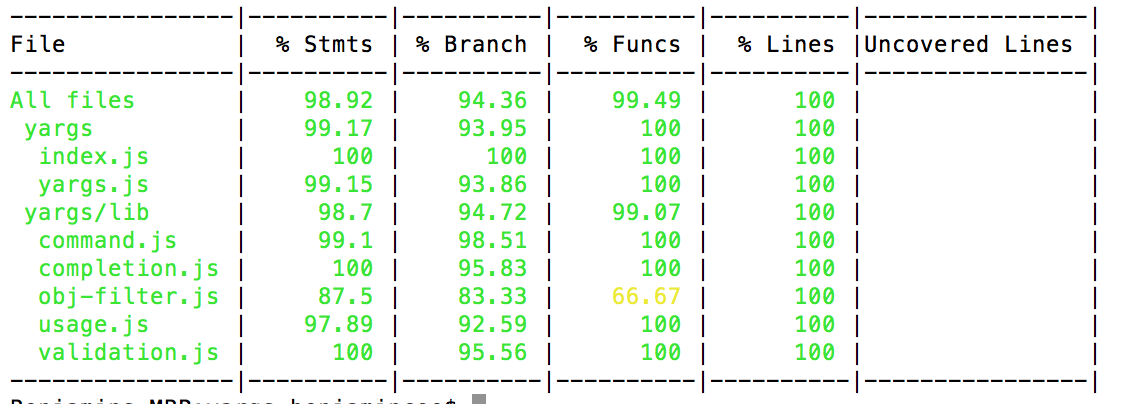
\includegraphics[width=0.9\textwidth]{CodeCoverage}
    \caption{A sample code coverage report}
    \end{figure}
\end{itemize}
\item CI will be set up using GitHub actions. The CI system will run automated tests triggered by a change to the main branch to ensure the main branch is always stable.
\begin{itemize}
    \item Mocha and Jest both have the necessary features needed to automate testing with GitHub actions.
\end{itemize}

\item Linter: \href{https://prettier.io/}{prettier}
\end{itemize}

\subsection{Software Validation Plan}


  One of the central purposes of this project is to gather research data through a user's gameplay. The supervisor, Prof. Niko Yiannakoulias, has done research before on the same topic, but through traditional survey methods instead of a game. The data obtained from his previous research will be important to validate the software, as it will help show if the software fulfilled its purpose of generating reliable data.
  \\ 

Another method of validating the software will be review sessions with our primary stakeholder, the supervisor (Prof. Niko Yiannakoulias). We have a weekly meeting cadence set up with him and we can use these to iteratively validate the software as we go through the development process as opposed to validating it just once. In the beginning, it will be best to keep these review sessions less formal but as the software gets closer to the finished product, the review sessions will become formal in nature and the group will implement task based inspection.

\section{System Test Description}
	
\subsection{Tests for Functional Requirements}
\label{s5.1}

% \wss{Subsets of the tests may be in related, so this section is divided into
%   different areas.  If there are no identifiable subsets for the tests, this
%   level of document structure can be removed.} \\
Game testing can be broken down into the following sections. The subsections will cover all the different components of the game. These components will work operate separately or work together to fulfill the functional requirements. Some of the components will be tested manually while others will require automated testing.


\subsubsection{Account Testing}

% \wss{It would be nice to have a blurb here to explain why the subsections below
%   cover the requirements.  References to the SRS would be good here.  If a section
%   covers tests for input constraints, you should reference the data constraints
%   table in the SRS.}
The account creation testing deals with the test cases related that relate to a user account. FR1, FR2, FR5 and FR15 are the functional requirements that are covered by the subsection. The system requires you to have an account to play the game. The test cases include the following: creating an account, resetting password, logging in, verifying if the user is human and account deletion.


%\subsubsubsection{Farm Testing}
%n/a
%\subsubsubsection{Shop Testing}
%n/a
%\subsubsubsection{Event Testing}
%n/a
%\subsubsection{User Decision Testing}
%n/a
%\subsubsection{User Account Testing}

\begin{enumerate}

%\item{GMTest-1\\}

%Control: Automatic
					
%Initial State: Camera is position at origin (x,y,z)  (0,0,0)
					
%Input: Move camera to the left
					
%Output: Camera's x position should only be changed and be translated  to the left by MOVE\_LEFT\_TEST units

%Test Case Derivation: \wss{Justify the expected value given in the Output field}
					
%How test will be performed: 


\item{\textbf{Name:} Successful Login } % FR 1

\textbf{Id:} Test-AC1 \label{Test-AC1} \\

\textbf{Control:} Automatic
					
\textbf{Initial State:} User is not logged in. Start at login page
					
\textbf{Input:} All valid information required for account creation
					
\textbf{Output:} Account corresponding to the input information is created in database with game state initialized to NEW\_ACCOUNT\_STATE

\textbf{Test Case Derivation:} To fully verify the account creation functionality, it is essential that the account information reflects the input information

\textbf{How test will be performed:} Create automatic test that creates an account and checks that the account can be logged into

\item{\textbf{Name:} Unsuccessful Login }% FR 1

\textbf{Id:} Test-AC2  \label{Test-AC2}\\

\textbf{Control: }Automatic
					
\textbf{Initial State:} User is not logged in and at login page
					
\textbf{Input:} At least 1 information required for account creation is invalid
					
\textbf{Output:} Account is not created in database and corresponding error is returned

\textbf{Test Case Derivation:} The system should not allow a user to create an account if they do not input all the necessary information, or if the information is invalid

\textbf{How test will be performed:} Create automatic test that inputs invalid information and verifies that a corresponding error is returned


\item{\textbf{Name:} Reset Password\\} \label{Test-AC3} % FR 2
\textbf{Id:} Test-AC3 \label{Test-AC3}\\

\textbf{Control:} Manual

\textbf{Initial State:} User is not logged in

\textbf{Input:} User's email

\textbf{Output:} Password was successfully reset

\textbf{Test Case Derivation:} In the event the user misplaces or forgets their password there needs to be a safeguard to ensure progress is not lost

\textbf{How test will be performed:} After resetting the password try to login with the new credentials to see if password was successfully reset


\item{\textbf{Name:} Verify Human User\\} % FR 5
\textbf{Id:} Test-AC4 \label{Test-AC4}\\

\textbf{Control: }Manual
					
\textbf{Initial State:} User is not logged in. Start at login page
					
\textbf{Input: }All information required for account creation is present
					
\textbf{Output: }System verifies user through a captcha

\textbf{Test Case Derivation: }Users must be able to succeed the captcha to ensure no automation of account creation is possible

\textbf{How test will be performed:} Manual test that fills in all account information and checks that a captcha is required before account creation is attempted

\item{\textbf{Name:} Successful deletion of user account\\} % FR 15
\textbf{Id:} Test-AC5    \label{Test-AC5}\\
\textbf{Control:} Manual
					
\textbf{Initial State:} User has an account and is logged in
					
\textbf{Input:} User request to have their account information deleted
					
\textbf{Output:} Data pertaining to the given username and password is deleted

\textbf{Test Case Derivation:} This functionality is essential for the ethics board and so must be thoroughly tested

\textbf{How test will be performed:} This test can be run after the other manual test of successfully creating an account

\end{enumerate}

\subsubsection{Game Mechanics Testing}
The game mechanics testing deals with the test cases related that relate to the game. FR3, FR4, FR6, FR7, FR8, FR9, FR10, FR11, FR12, FR16, FR17, FR19, FR21 and FR22 are the functional requirements that are covered by the subsection. The game mechanics compose of all the game logic and consist of any actions the player is able to perform in the context of the game. Examples of these test cases include successfully buying and selling crops.

\begin{enumerate}




% \noindent\textbf{\\User Currency}
% \item{test-uc1\\} % FR 3
% Control: Manual
					
% Initial State: User is logged in and at game page
					
% Input: Any action that increases an account's currency
					
% Output: Currency correctly reflects the outcome of selling items, in both the database and front-end

% Test Case Derivation: User's should always accurately be aware of how much money they have to ensure they make genuine and calculated decisions within the game

% How test will be performed: Thorough and iterative manual testing of the selling functionality

% \item{test-uc2\\} % FR 3
% Control: Manual
					
% Initial State: User is logged in and at game page
					
% Input: Any action that decreases an account's currency
					
% Output: Currency correctly reflects the outcome of buying items, in both the database and front-end

% Test Case Derivation: User's should always accurately be aware of how much money they have to ensure they make genuine and calculated decisions within the game

% How test will be performed: Thorough and iterative manual testing of the buying functionality



\item {\textbf{Name:} Successful first item purchase\\} % FR 3, 6
\textbf{Id:} Test-GM1 \label{Test-GM1}\\

Control: Automatic

\textbf{Initial State:} User is logged in and in the shop. User has enough in-game currency to purchase an item but does not have the item in their inventory

\textbf{Input:} User is logged in. The user buys an item

\textbf{Output:} The item appears in the user's inventory and the user's currency correctly reflects the outcome of buying items

\textbf{Test Case Derivation:} The system must be able to verify that users can purchase a new item they do not currently own using in-game currency

\textbf{How test will be performed:} Automated test to check if purchased item exists in inventory and the user's currency is correctly reflected after the purchase, in both the database and front-end

\item {\textbf{Name:} Unsuccessful item purchase\\} % FR 3, 6
\textbf{Id:} Test-GM2 \label{Test-GM2}\\

\textbf{Control:} Automatic

\textbf{Initial State:} User is logged in and in the shop. User does not have enough in-game currency to purchase an item but does not have the item in their inventory

\textbf{Input:} The user buys an item

\textbf{Output:} The item does not appear in the user's inventory and the user's currency is not changed

\textbf{Test Case Derivation:} The system must be able to verify that users can not purchase an item using in-game currency when they do not have enough in-game currency

\textbf{How test will be performed:} Automated test to check if the user has enough in-game currency to purchase that item which does not change after an unsuccessful purchase, in both the database and front-end

\item {\textbf{Name:} Successful second or more item purchase of the same item\\} % FR 3, 6
\textbf{Id:} Test-GM3 \label{Test-GM3}\\

\textbf{Control:} Automatic

\textbf{Initial State:} User is logged in and in the shop. User has enough in-game currency to purchase an item and already has the item in their inventory

\textbf{Input:} The user buys an item they already have in their inventory 

\textbf{Output:} The quantity of the same item is increased by 1 in the user's inventory and the user's currency correctly reflects the outcome of buying items

\textbf{Test Case Derivation: }The system must be able to verify that users can purchase items to use for farming purposes

\textbf{How test will be performed:} Automatic test to check if purchased item count in inventory has increased and the user’s currency is correctly reflected after the purchase, in both the database and front-end

\item{\textbf{Name:} Successful Land Purchase\\} % FR 3, FR 7, FR 17, FR 10
\textbf{Id:} Test-GM4 \label{Test-GM4}\\

\textbf{Control:} Manual
					
\textbf{Initial State:} User is logged in and at game page
					
\textbf{Input:} User requests to buy selected land area
					
\textbf{Output:} User's currency count correctly reflects the price of buying the land, and the user is able to interact with new bought piece of land

\textbf{Test Case Derivation:} User's should always accurately be aware of how much money they have to ensure they make genuine and calculated decisions within the game, and be able to expand their farm

\textbf{How test will be performed:} Thorough and iterative manual testing of the land functionality

\item{\textbf{Name:} Successful planting of seeds\\} % FR4, FR 7, FR 17
\textbf{Id:} Test-GM5 \label{Test-GM5}\\

\textbf{Control:} Manual
					
\textbf{Initial State:} User is logged in, at game page, and has an empty piece of land
					
\textbf{Input: }User requests to plant seeds on selected land area
					
\textbf{Output:} The seeds are removed from the user's inventory and planted on the selected area

\textbf{Test Case Derivation:} User's should always accurately be aware of what is in their inventory and be able to plant crops

\textbf{How test will be performed: }Thorough and iterative manual testing of the farming functionality

\item{\textbf{Name:} Successful growing of plant seeds\\} % FR 7
\textbf{Id:} Test-GM6 \label{Test-GM6}\\

\textbf{Control:} Manual
					
\textbf{Initial State:} User is logged in, at game page, and has planted a seed on a piece of land
					
\textbf{Input:} User ends turn
					
\textbf{Output:} All planted seeds grow by 1 turn

\textbf{Test Case Derivation:} User's should be able to plant crops and know of a plant's growth progress

\textbf{How test will be performed:} Thorough and iterative manual testing of the farming functionality

\item{\textbf{Name:} Selling the same crop in different seasons\\} % FR 8 
\textbf{Id:} Test-GM7 \label{Test-GM7}\\

\textbf{Control: }Automatic

\textbf{Initial State:} User is logged in, user is at the shop, and the user owns at least two of the same crop

\textbf{Input:} User sells the one of the crops in current season and the other in the next season

\textbf{Output:} Profit earned from selling the two of the same crops in different seasons should vary 

\textbf{Test Case Derivation:} The user should be able to somewhat simulate a real market where crops can be sold at varying prices at different times and market

\textbf{How the test will be performed:} Automated test to sell two of the same crops during different time periods and ensure the prices are the different to check for random sell prices

\item{\textbf{Name:} Selling the same crop in same seasons\\} % FR 8 
\textbf{Id:} Test-GM8 \label{Test-GM8}\\

\textbf{Control: }Automatic

\textbf{Initial State:} User is logged in, user is at the shop, and the user owns at least two of the same crop

\textbf{Input:} User sells the one of the crops in current season and the other in the next season

\textbf{Output:} Profit earned from selling the two of the same crops in the same seasons should be the same 

\textbf{Test Case Derivation:} The user should be able to somewhat simulate a real market where crops can be sold at varying prices at different times and market

\textbf{How the test will be performed:} Automated test to sell two of the same crops during the same time periods and ensure the prices are the same to check for random sell prices

\item{\textbf{Name:} Successful balance increase in selling crop\\} % FR 8 
\textbf{Id:} Test-GM9 \label{Test-GM9}\\

\textbf{Control:} Automatic

\textbf{Initial State:} User is logged in and at the shop

\textbf{Input:} Crop to be sold

\textbf{Output:} Money earned through selling crop. User's currency count correctly reflects the increase in user's currency count


\textbf{Test Case Derivation:} The user should be able to somewhat simulate a real market where crops can be sold at varying prices depending on the time and market

\textbf{How the test will be performed:} Automatic test to check if user's money/balance has increased after selling a crop

\item{\textbf{Name:} Successful decrease in item quantity after selling item\\} % FR 8 
\textbf{Id:} Test-GM10 \label{Test-GM10}\\

\textbf{Control:} Automatic

\textbf{Initial State:} User is logged in, at the shop, and holds at least one crop in inventory

\textbf{Input:} User sells one crop

\textbf{Output:} The inventory count decreases by one and money earned through the sale is added to the user's in-game currency balance

\textbf{Test Case Derivation:} The user should no longer have the same number of items once its sold

\textbf{How the test will be performed: }Automatic test to check if crop that has been sold has been removed from the inventory


\item{\textbf{Name:} Successful use of fertilizer on crop\\} % FR 7, FR 9, FR 17
\textbf{Id:} Test-GM11 \label{Test-GM11}\\

\textbf{Control:} Manual
					
\textbf{Initial State: }User is logged in, at game page, and has planted a seed on a piece of land
					
\textbf{Input:} User requests to use fertilizer on a selected planted seed
					
\textbf{Output: }Planted seed's growth is accelerated by FERTILIZER\_EFFECT

\textbf{Test Case Derivation:} User's should be able to use fertilizer on crops to create a more complex decision making system

\textbf{How test will be performed:} Thorough and iterative manual testing of the farming functionality

\item{Name: Successful visual check of farm area enlarged\\} % FR 10 FR16
\textbf{Id:} Test-GM12 \label{Test-GM12}\\

\textbf{Control:} Manual

\textbf{Initial State:} User is logged in and is in the shop

\textbf{Input:} Amount of land to be purchased

\textbf{Output:} The land is purchased and the farm area is larger prior to purchase that the user can interact with

\textbf{Test Case Derivation: }The game should be somewhat expansive and the user should be able to purchase land to enlarge their farm

\textbf{How the test will be performed: }Manual test to check visually if the farm area has enlarged

\item{\textbf{Name:} Successful purchase of building\\} % FR 17
\textbf{Id:} Test-GM13 \label{Test-GM13}\\

\textbf{Control:} Manual
					
\textbf{Initial State:} User is logged in, at game page, and has an empty piece of land
					
\textbf{Input:} User requests to buy and place building on selected land tile
					
\textbf{Output:} User's currency count correctly reflects the price of buying the building and the building is placed on the selected tile

\textbf{Test Case Derivation:} User's should be able to buy and place buildings to create a more complex decision making system

\textbf{How test will be performed: }Thorough and iterative manual testing of the farming functionality

\item{\textbf{Name:} Successful evaluate all users asset in inventory\\} % FR 19
\textbf{Id: }Test-GM14 \label{Test-GM14}\\

\textbf{Control:} Automatic
					
\textbf{Initial State:} User is logged in and at game page
					
\textbf{Input:} User requests to have their farm evaluated
					
\textbf{Output:} Total worth of a user's assets % and a star ranking corresponding to the STAR\_MILESTONES

\textbf{Test Case Derivation:} User's should be able to visualize their progression to help in their decision-making and engagement

\textbf{How test will be performed:} Evaluate all assets in the users inventory


\item{\textbf{Name:} Automatic prompt for a consultant\\} % FR 11
\textbf{Id:} Test-GM15 \label{Test-GM15} \\

\textbf{Control:} Manual
					
\textbf{Initial State:} User is logged in and at game page
					
\textbf{Input:} User progresses to a turn number that is divisible by CONSULTING\_INTERVAL
					
\textbf{Output:} User is prompted on whether or not they want to pay for consulting advice

\textbf{Test Case Derivation:} This prompt is essential to the research study aspect of the system, which must be functional and consistent in order for the research to propose a conclusion

\textbf{How test will be performed:} Manual testing of playing the overall game and ensuring the consultant prompt would be present every CONSULTING\_INTERVAL turns

\item{\textbf{Name:} Consultant's advice\\} % FR 11 FR 20
\textbf{Id:} Test-GM16 \label{Test-GM16}\\

\textbf{Control:} Manual
					
\textbf{Initial State:} User is logged in and at game page
					
\textbf{Input:} User plays the game for multiple turns and is prompted on whether or not they want to pay for consulting advice
					
\textbf{Output:} The consulting advice is randomly given as either deterministic or probabilistic

\textbf{Test Case Derivation:} This distinction between deterministic and probabilistic information is essential to the research study aspect of the system, which must be functional and consistent in order for the research to propose a conclusion. The same type of advice should be given a each player throughout the game

\textbf{How test will be performed:} Manual testing of playing the overall game and ensuring the consultant information is either deterministic or probabilistic on average 50\% of the time for each

\item{\textbf{Name:} Successful prompt for insurance upon purchasing a crop\\} % FR 12 FR 20 <- Confirm insurance can only be purchased in shop
\textbf{Id:} Test-GM17 \label{Test-GM17}\\

\textbf{Control:} Manual 

\textbf{Initial State:} User is logged in and in shop

\textbf{Input:} User is prompted on whether or not they will purchase insurance with the crop.

\textbf{Output:} Insurance is added to crop in case of damage

\textbf{Test Case Derivation:} The research also aims to understand if user's are willing to pay for insurance and under what circumstance.

\textbf{How test will be performed:} Manual test to check whether prompt appears to purchase insurance when purchasing a crop.

\item{\textbf{Name:} Successful occurrence of random events/decisions happening twice in one season\\} % FR 21
\textbf{Id:} test-GM18 \label{Test-GM18}\\

\textbf{Control:} Manual
					
\textbf{Initial State: }User is logged in and at game page
					
\textbf{Input:} User plays out 1 season, of which is equivalent to SEASON\_LENGTH amount of turns
					
\textbf{Output:} User is prompted with a random event EVENT\_OCCURRENCE amount of times within that season

\textbf{Test Case Derivation:} This functionality is essential to the study as these decoy decisions/events hide the decisions that matter to the research. These decoy decisions ensure participants are unaware of what they actual study is about and so must be thoroughly tested

\textbf{How test will be performed:} Manual testing of playing the overall game and ensuring these random events/decisions happen twice a season

\item{\textbf{Name:} Successful season change\\} % FR 22
\textbf{Id:} Test-GM19 \label{Test-GM19}\\

\textbf{Control:} Automated

\textbf{Initial State:} User has played the game for some time

\textbf{Input:} User has played SEASON\_LENGTH turns

\textbf{Output:} the state of the season change

\textbf{Test Case Derivation:} This is significant as it will encourage the user to plan ahead and try to optimize their decisions in the game for the best outcomes.

\textbf{How the test will be performed:} Automated test to check whether after SEASON\_LENGTH the season has changed.

\item{\textbf{Name: }Successful visual season change\\} % FR 22
\textbf{Id:} test-GM20 \label{Test-GM20}\\

\textbf{Control:} Manual

\textbf{Initial State:} User has played the game for some time

\textbf{Input:} Any decisions the user has made ?

\textbf{Output:} Season change

\textbf{Test Case Derivation: }This is significant as it will encourage the user to plan ahead and try to optimize their decisions in the game for the best outcomes.

\textbf{How the test will be performed:} Manual test by playing the game for some time and visually checking whether the season is changing or remains constant.

\item{\textbf{Name:} Item successfully added to inventory \\} % FR 4 
\textbf{Id:} test-GM21 \label{Test-GM21}\\

\textbf{Control:} Automatic

\textbf{Initial State:} User is logged in and inventory is Empty

\textbf{Input:} add item to inventory

\textbf{Output:} item successfully added to inventory and inventory is not empty

\textbf{Test Case Derivation:} The system must be able to check if items can be stored in the inventory to allow users to view them

\textbf{How test will be performed: }Create automatic test that check that the inventory object is not empty when an item is added

\end{enumerate}

\subsubsection{Database Testing}
The database testing deals with the test cases related that relate to the game. FR13 and FR14 are the functional requirements that are covered by the subsection. The database is critical as it will log decisions and the game state. The test cases ensure that the game decisions and game state will be successfully logged.
\begin{enumerate}

\item{\textbf{Name:} Logging game decisions\\} % FR 13
\textbf{Id:} Test-DB1    \label{Test-DB1}\\
\textbf{Control:} Manual
					
\textbf{Initial State:} User is logged in and at game page
					
\textbf{Input:} Any action the user performs while playing the game
					
\textbf{Output: }All actions will be logged

\textbf{Test Case Derivation:} The research is highly dependent on decisions which are the actions that will be logged by the game.

\textbf{How test will be performed:} Manual test by checking the server logs to see if all actions are being logged.

% Not game mechanics
\item{\textbf{Name:} Successful saving of game state\\} % FR 14
\textbf{Id:} Test-DB2    \label{Test-DB2}\\
\textbf{Control:} Manual

\textbf{Initial State:} User is logged in and makes a turn to change the game state.

\textbf{Input:} The user will be able to select an option to save

\textbf{Output:} The new game state will be saved

\textbf{Test Case Derivation:} The user needs to have the option of being able to continue where they left off in case they wish to play at a later time.

\textbf{How the test will be performed:} Manual test to perform an action(eg. buy an item) and checking whether the game state is saved. The test will save after the action and log out then log back in to check if saving was successful. 

\subsubsection{Pre-Game Testing}
The Pre-game testing deals with the test cases related that relate to the user before they can start playing the game. FR18 is the only functional requirement that is covered by the subsection. To play the game, the user must agree to the terms and conditions in the consent form. 

\item{\textbf{Name:} User agrees to the consent form\\} %FR 18
\textbf{Id:} Test-PG1 \label{Test-PG1}\\

\textbf{Control:} Automatic

\textbf{Initial State:} User is not logged in, has not played the game yet, and is presented the consent form

\textbf{Input:} The user accepts the terms and conditions to the consent form

\textbf{Output:} User is re-directed to the login screen

\textbf{Test Case Derivation:} This is mandatory to conduct the study and without the user's consent their data will not be able to be collected

\textbf{How the test will be performed:} Automated test to check if all terms and conditions to play the game have been met


\item{\textbf{Name:} User does not agree to consent form\\} %FR 18
\textbf{Id:} Test-PG2 \label{Test-PG2}\\

\textbf{Control:} Automatic

\textbf{Initial State:} User is not logged in, has not played the game yet, and is presented the consent form

\textbf{Input:} The user rejects the terms and conditions to the consent form

\textbf{Output:} The user is unable to access the login screen and play the game

\textbf{Test Case Derivation:} This is mandatory to conduct the study and without the user's consent their data will not be able to be collected

\textbf{How the test will be performed:} Automated test will reject the consent form and try to access the login screen


\end{enumerate}
\subsection{Tests for Nonfunctional Requirements}
\label{s5.2}

% \wss{The nonfunctional requirements for accuracy will likely just reference the
%   appropriate functional tests from above.  The test cases should mention
%   reporting the relative error for these tests.  Not all projects will
%   necessarily have nonfunctional requirements related to accuracy}

% \wss{Tests related to usability could include conducting a usability test and
%   survey.  The survey will be in the Appendix.}

% \wss{Static tests, review, inspections, and walkthroughs, will not follow the
% format for the tests given below.}
The non-functional system requirements that require non-functional testing. These tests can be broken down into different subsections that cover the areas of testing. These subsections for the non-functional tests include: Look and Feel, Usability and Humanity, Performance, Operational and Environmental, Maintainability and Support Requirements, Security, Access and Integrity.
Area of Testing:
\begin{itemize}
    \item Client Side \& Server Side Performance Testing
    \item Security \& Data Integrity Testing
    \item Look and Feel 
    \item Usability
\end{itemize}


\subsubsection{Look and Feel}

\begin{enumerate}

\item{\textbf{Name:} Survey for feedback on different interface elements\\} \label{Test-LF1}% 
\textbf{Id:} Test-LF1\\

\textbf{Type:} Non-functional, Dynamic, Manual
					
\textbf{Initial State: }The user is at home page
					
\textbf{Input:} The user registers account, logs in and plays out one season
					
\textbf{Output/Result:} Get feedback and verify interface is not overwhelming
					
\textbf{How test will be performed:} A survey will be given to the players where they will give feedback to different elements of the interface.
					
\item{\textbf{Name: }Test the system on different screen resolutions \\}\label{Test-LF2}
\textbf{Id: }Test-LF2\\

\textbf{Type: }Non-functional, Dynamic, Manual
					
\textbf{Initial State:} The user is at home page
					
\textbf{Input:} The user registers account, logs in and plays out one season
					
\textbf{Output:} Get feedback and verify interface is clear at different SCREEN\_RESOLUTION %The user is prompted to navigate to different screens and accesses different interface features.
					
\textbf{How test will be performed:} The test will be performed manually with the tester playing one season at different SCREEN\_RESOLUTION in which they are to navigate to different screens and access different interface features.

\item{\textbf{Name: }Testing User Engagement \\}\label{Test-LF3}
\textbf{Id: }Test-LF3\\

\textbf{Type:} Non-functional, Dynamic, Automated
					
\textbf{Initial State:} The user is logged into the game
					
\textbf{Input:} The user plays the game
					
\textbf{Output: }Have metric of how engaged the player is depending on how many turns they play in a session
					
\textbf{How test will be performed:} The user decisions and the number of turns played are logged and the total number of turns played will be calculated for every player and compared to MIN\_TURNS. If player has played greater than or equal to MIN\_TURNS, we say they were engaged.


\end{enumerate}

\subsubsection{Usability and Humanity}
\begin{enumerate}
    \item{\textbf{Name: }Testing Learnability\\}\label{Test-UH1}
    \textbf{Id: }Test-UH1\\


    \textbf{Type: }Non-functional, Dynamic, Manual
    					
    \textbf{Initial State:} The user is at home page
    					
   \textbf{Input: }The user registers account, logs in and plays the game
    					
   \textbf{Output:} Get feedback and verify authorization, game logic, and interface is easy/fast to learn
    					
    \textbf{How test will be performed: }A survey will be given to players to provide feedback on how easy it is to learn the different aspects of the system. This includes the game logic and interactions between the different menus
\end{enumerate}

\subsubsection{Performance}
\begin{enumerate}
    \item{\textbf{Name: }Test the load times for logging the game\\}\label{Test-P1}
    \textbf{Id: }Test-P1\\
    
    \textbf{Type:} Non-functional, Automated, Dynamic
    					
    \textbf{Initial State: }The game server is online and running, user is at home page
    					
    \textbf{Input:} The user logs into the game
    					
   \textbf{Output: }The user is able to log into the game within LOAD\_TIME
    					
   \textbf{How test will be performed:} The team will use a performance testing tool of choice to measure loading times of logging in to the game.
    
    
    %%% WONDERING IF WE CAN INCLUDE P2, (IR1, IR2 from hazard) into 1 test
    \item{\textbf{Name: }Test response time of the system based on user input\\}\label{Test-P2}
     \textbf{Id: }Test-P2\\
    
    \textbf{Type: }Non-functional, Automated, Dynamic
    					
    \textbf{Initial State:} The user is logged into the game
    					
    \textbf{Input:} The user makes a decisions within the game and interacts with the user interface
    					
    \textbf{Output:} The application provides a response to the request within RESPONSE\_TIME
    					
    \textbf{How test will be performed:} The team will use a performance testing tool of choice to measure the response times of different decisions within the game.


\item{\textbf{Name:} Test for performance on using different image assets \\}\label{Test-P3}
\textbf{Id: }Test-P3\\

\textbf{Type:} Automated, Dynamic
					
\textbf{Initial State:} The user is logged into the game
					
\textbf{Input: }An existing image asset is replaced
					
\textbf{Output:} The new image can be seen in place of the replaced image asset and the application response does not exceed RESPONSE\_TIME
					
\textbf{How test will be performed: }The team will use a performance tool of choice to automate replacing an image asset and measuring the response time of different interface interactions.
\end{enumerate}

\subsubsection{Operational and Environmental}
\begin{enumerate}
    %%% Double check that we can involve multiple system/unit test in 1 test to test the whole functionality of the system through automated testing
    %%% If not, just make this manual testing
    \item{\textbf{Name: }Testing if system can run on different browsers\\} \label{Test-OE1}
    \textbf{Id: }Test-OE1\\
    
   \textbf{Type:} Non-functional, Automated, Dynamic
    					
    \textbf{Initial State:} The user is at home page
    					
   \textbf{Input:} The user registers account, logs in and plays the game on different modern web browsers
    					
   \textbf{Output: }The system shall be functional with no errors
    					
   \textbf{How test will be performed: }The system will be tested with various features of the system in order to determine the system is working correctly on different modern web browsers. This will ensure the system can be supported by that specific web browser.
    
    \item{\textbf{Name: }Test for all working versions of a web browser up to supported working version \\} \label{Test-OE2}
    \textbf{Id: }Test-OE2\\
    
    \textbf{Type:} Non-functional, Automated, Dynamic
    					
    \textbf{Initial State: }The user is at home page
    					
   \textbf{Input:} The user registers account, logs in and plays the game on different versions of different modern web browsers
    					
    \textbf{Output:} The system shall be functional with no errors
    					
    \textbf{How test will be performed:} The system will be tested with various features of the system in order to determine the system is working correctly on different versions of that web browser. The system will test from the SUPPORTED\_VERSION to the latest version of that web browser
\end{enumerate}

\subsubsection{Maintainability and Support Requirements}
\begin{enumerate}
\item{\textbf{Name:} Testing audio change in current game session and its affects\\}\label{Test-MS1}
\textbf{Id:} Test-MS1\\

\textbf{Type:} Non-functional, Manual, Dynamic
					
\textbf{Initial State:} The user is logged into the game
					
\textbf{Input:} The game audio is changed to a different track 
					
\textbf{Output:} The change is game audio does not affect other aspects of the game
					
\textbf{How test will be performed:} A member of the team will switch the game audio to a different track and monitor the effect on the game after the change.
\end{enumerate}



\subsubsection{Security}
\begin{enumerate}
    \item{\textbf{Name:} Test for exploits of current technology used in the system\\} \label{Test-SR1}
   \textbf{Id: }Test-SR1\\
   
    \textbf{Type:} Non-functional, Manual, Dynamic
    					
    \textbf{Initial State:} The user is not logged in
    					
    \textbf{Input:} User creates account
    					
    \textbf{Output:} The system shall prevent the creation of accounts in suspicion of automated attacked
    					
    \textbf{How test will be performed:} Use common exploit vulnerabilities with the current versions or past versions of the technology used within the system that can lead to automated attacks. This will be used on a separate test server to avoid any complications with the development server.
    
    \item{\textbf{Name:} Test for basic cross site scripting (XSS) to by pass login screen\\} \label{Test-SR2}
    \textbf{Id:} Test-SR2\\
    
    \textbf{Type:} Non-functional, Manual, Dynamic
    					
    \textbf{Initial State:} The user is not logged in
    					
    \textbf{Input:} User logins
    					
    \textbf{Output:} The system shall prevent user from logging in through malicious attack
    					
    \textbf{How test will be performed:} Basic cross site scripting (XSS) techniques will be used to see if the user is able to by-pass the login screen. Some techniques include persistent, non-persistent and DOM-based cross-site scripting.
    
    % \item{\textbf{Id:} Test-SR3\\} \label{Test-SR3}
    
    % \textbf{Type:} Non-functional, Manual, Dynamic
    					
    % \textbf{Initial State:} The user is not logged in
    					
    % \textbf{Input:} User logins
    					
    % \textbf{Output:} The system shall prevent a verified user from allowing multiple instances of the same account to run
    					
    % \textbf{How test will be performed:} Logging on multiple instances on the same web browser, opening multiple instances on the different browsers on the same device, opening multiple instances on different devices and on different browsers.
    
    \item{\textbf{Name:} Test to see if plain text of password exist in database\\} \label{Test-SR3}
    \textbf{Id:} Test-SR3\\
    
    \textbf{Type:} Non-functional, Manual, Dynamic
    					
    \textbf{Initial State:} Only one user's password is encrypted in data base and admin access to data base
    					
    \textbf{Input:} Query passwords for passwords in database
    					
    \textbf{Output:} Encrypted user password
    					
    \textbf{How test will be performed:} Manually query the passwords in the data base and check to see if the user password is returned in plaintex
\end{enumerate}

\subsubsection{Access}
\begin{enumerate}
    \item{\textbf{Name:} Test for accessing the system on different internet accesses (i.e public and private wifi)\\} \label{Test-ACR1}
    \textbf{Id:} Test-ACR1\\
    
    \textbf{Type:} Non-functional, manual, Dynamic
    					
    \textbf{Initial State:} The user is not logged in
    					
    \textbf{Input:} User accesses system
    					
    \textbf{Output:} The system successfully loads on users system
    					
    \textbf{How test will be performed:} The system will be opened on multiple systems in multiple locations (i.e public, private internet access and check to see if the system is able to be accessed by the user. However, only one user session is active at a time.
    
    \item{\textbf{Name:} Test to see if only login functionality is only provided when user is not logged in\\} \label{Test-ACR2}
    \textbf{Id:} Test-ACR2\\
    
    \textbf{Type:} Non-functional, manual, Dynamic
    					
    \textbf{Initial State:} The user is not logged in and at login page
    					
    \textbf{Input:} N/A
    					
    \textbf{Output:} The system will only provide functionality relating to logging in. The system should not allow any functionality relating to the in-game subsystem when they are not logged in.
    					
    \textbf{How test will be performed:} The system checked to see which request are provided when presented at the login screen when the user is not signed in. There will be checks to see if any game related logic is stored on the user's client side to see if they have access to functionality they should not be having access to while not signed in. 
    
    \item{\textbf{Name:} Test to see if only in game functionality is provided when user is logged in (i.e functionality for logging should not be available)\\} \label{Test-ACR3}
    \textbf{Id: }Test-ACR3\\
    
    \textbf{Type:} Non-functional, manual, Dynamic
    					
    \textbf{Initial State:} The user is logged in and at game page
    					
    \textbf{Input:} N/A
    					
    \textbf{Output:} The system will provide all functionality relating to the game upon after logging. All functionality related to the login should not be present 
    					
    \textbf{How test will be performed:} The system checked to see which request are provided after the user is logged in and at the game page. There will be checks to see if all game related logic is stored on the user's client side after they are logged in and playing the game. There should be no functionality related to the login system 
    
    \item{\textbf{Name:} Test to see if only one user session is activated each time a new log in appears\\} \label{Test-ACR4}
    \textbf{Id: }Test-ACR4\\
    
    \textbf{Type:} Non-functional, manual, Dynamic
    					
    \textbf{Initial State:} The user is logged in and at game page in one session
    					
    \textbf{Input:} User attempts to login into a separate session
    					
    \textbf{Output:} The system shall only allow the new session created by the user upon login to a new session to be active while deactivating the previous user session
    					
    \textbf{How test will be performed:} Have one session logged in and sign in again in a different tab/window on the same machine and testing on a separate machine. Each instance of this test, only one session should be active while deactivating the previous user session 
    
\end{enumerate}

\subsubsection{Integrity}
\begin{enumerate}
    \item{\textbf{Name:} Testing API Response Time \\} \label{Test-IR1}
    \textbf{Id:} IR1 \\
    
    \textbf{Type:} Non-functional, Automatic, Dynamic
    					
    \textbf{Initial State:} The user is logged in
    					
    \textbf{Input:} User plays the game
    					
    \textbf{Output:} The system shall respond with user input request
    					
    \textbf{How test will be performed:} The system shall be able to receive all input request provided by the user and each one takes at most API\_RESPONSE\_TIME
    
    \item{\textbf{Name:} Testing Database Response Time \\} \label{Test-IR2}
    \textbf{Id:} IR2 \\
    
    \textbf{Type:} Non-functional, Automatic, Dynamic
    					
    \textbf{Initial State:} N/A
    					
    \textbf{Input:} System makes request to database
    					
    \textbf{Output:} The database shall respond to system request
    					
    \textbf{How test will be performed:} The database will receive all types of input requests provided by the system and each one takes at most DATABASE\_RESPONSE\_TIME
    
    \item{\textbf{Name:} Testing if progress is saved when connection is lost \\} \label{Test-IR3}
    \textbf{Id:} IR3 \\
    
    \textbf{Type:} Non-functional, Manual, Dynamic
    					
    \textbf{Initial State:} User logged in
    					
    \textbf{Input:} User disconnects from internet
    					
    \textbf{Output:} The system shall keep user progress prior to loss of connection and resume gameplay upon an established connection with the server
    					
    \textbf{How test will be performed:} The user will disconnect their game mid session (i.e disconnect internet, close tab, web browser client) and then reconnect and log back into their game. Check to see if progress prior to loss of connection was saved and resumed
\end{enumerate}

\subsection{Traceability Between Test Cases and Requirements}


\subsubsection{Traceability Matrix for Functional Requirement Test Cases}

\begin{table}[H]
\begin{adjustwidth}{-1.57in}{-1in}
\resizebox{8.5in}{!}{\begin{tabular}{c|c|c|c|c|c|c|c|c|c|c|c|c|c|c|c|c|c|c|c|c|c|c|}
\cline{2-23}
                                    & \textbf{FR1} & \textbf{FR2} & \textbf{FR3} & \textbf{FR4}  & \textbf{FR5} & \textbf{FR6} & \textbf{FR7} & \textbf{FR8} & \textbf{FR9} & \textbf{FR10} &\textbf{FR11} & \textbf{FR12} & \textbf{FR13} & \textbf{FR14}& \textbf{FR15}& \textbf{FR16}& \textbf{FR17}& \textbf{FR18} & \textbf{FR19}& \textbf{FR20}& \textbf{FR21}& \textbf{FR22} \\ \hline
\multicolumn{1}{|c|}{\hyperref[Test-AC1]{\textbf{AC1}}}  &       X       &              &              &              &              &              &              &              &              &              &              &              &             &              &             &             &             &        & & & &     \\ \hline
\multicolumn{1}{|c|}{\hyperref[Test-AC2]{\textbf{AC2}}}  &      X        &              &              &              &              &              &              &              &              &              &              &              &              &              &             &             &             &        & & & &      \\ \hline
\multicolumn{1}{|c|}{\hyperref[Test-AC3]{\textbf{AC3}}}  &              &      X        &              &              &              &             &              &              &              &              &              &              &              &              &             &             &             &      & & & &        \\ \hline
\multicolumn{1}{|c|}{\hyperref[Test-AC4]{\textbf{AC4}}}  &              &              &              &              &      X        &              &              &              &              &              &              &              &              &              &             &             &             &        & & & &      \\ \hline
\multicolumn{1}{|c|}{\hyperref[Test-AC4]{\textbf{AC5}}}  &              &              &              &              &              &              &              &              &              &              &              &              &              &              &    X         &             &             &        & & & &      \\ \hline
\multicolumn{1}{|c|}{\hyperref[Test-GM1]{\textbf{GM1}}}  &              &              &       X       &              &              &          X    &              &              &              &              &              &              &              &              &             &             &             &        & & & &      \\ \hline
\multicolumn{1}{|c|}{\hyperref[Test-GM2]{\textbf{GM2}}}  &              &              &        X      &              &              &         X    &              &              &              &              &              &              &              &              &             &             &             &       & & & &       \\ \hline
\multicolumn{1}{|c|}{\hyperref[Test-GM3]{\textbf{GM3}}}  &              &              &         X     &              &              &       X      &              &              &              &              &              &              &              &              &             &             &             &       & & & &       \\ \hline
\multicolumn{1}{|c|}{\hyperref[Test-GM4]{\textbf{GM4}}}  &              &              &       X       &              &              &             &    X          &              &              &       X       &              &              &              &              &             &      X       &    X         &       & & & &       \\ \hline
\multicolumn{1}{|c|}{\hyperref[Test-GM5]{\textbf{GM5}}}  &              &              &              &       X       &              &             &     X         &              &              &              &              &              &              &              &             &             &       X      &         & & & &     \\ \hline
\multicolumn{1}{|c|}{\hyperref[Test-GM6]{\textbf{GM6}}} &              &              &              &              &              &             &        X      &              &              &              &              &              &              &              &             &             &             &         & & & &     \\ \hline
\multicolumn{1}{|c|}{\hyperref[Test-GM7]{\textbf{GM7}}} &              &              &              &              &              &              &              &      X        &              &              &              &              &              &              &             &             &             &         & & & &     \\ \hline
\multicolumn{1}{|c|}{\hyperref[Test-GM8]{\textbf{GM8}}} &              &              &              &              &              &              &              &       X       &              &              &              &              &              &              &             &             &             &          & & & &    \\ \hline
\multicolumn{1}{|c|}{\hyperref[Test-GM9]{\textbf{GM9}}} &              &              &              &              &              &              &              &      X        &              &              &              &              &              &              &             &             &             &         & & & &     \\ \hline
\multicolumn{1}{|c|}{\hyperref[Test-GM10]{\textbf{GM10}}} &              &              &              &              &              &              &              &     X         &              &              &              &              &              &              &             &             &             &           & & & &   \\ \hline
\multicolumn{1}{|c|}{\hyperref[Test-GM11]{\textbf{GM11}}} &              &              &              &              &              &              &       X       &              &        X      &              &              &              &              &             &             &            &       X      &            & & & &  \\ \hline
\multicolumn{1}{|c|}{\hyperref[Test-GM12]{\textbf{GM12}}} &              &              &              &              &              &             &              &              &              &      X        &              &              &              &              &             &           X  &             &            & & & &  \\ \hline
\multicolumn{1}{|c|}{\hyperref[Test-GM13]{\textbf{GM13}}} &              &              &              &              &              &             &              &              &              &              &              &              &              &              &             &             &        X     &           & & & &   \\ \hline
\multicolumn{1}{|c|}{\hyperref[Test-GM14]{\textbf{GM14}}} &              &              &              &              &              &              &              &              &              &              &              &              &              &              &             &            &             &           &X & & &   \\ \hline
\multicolumn{1}{|c|}{\hyperref[Test-GM15]{\textbf{GM15}}} &              &              &              &              &              &              &              &              &              &              &   X           &              &              &              &             &             &             &          & & & &    \\ \hline
\multicolumn{1}{|c|}{\hyperref[Test-GM16]{\textbf{GM16}}} &              &              &              &              &              &              &              &              &              &              &    X          &              &              &              &             &             &             &          & &X & &    \\ \hline
\multicolumn{1}{|c|}{\hyperref[Test-GM17]{\textbf{GM17}}} &              &              &              &              &              &             &              &              &              &              &              &     X         &              &              &             &             &             &           & &X & &   \\ \hline
\multicolumn{1}{|c|}{\hyperref[Test-GM18]{\textbf{GM18}}} &              &              &              &              &              &              &              &              &              &              &              &              &              &              &             &             &             &           & & & X&   \\ \hline
\multicolumn{1}{|c|}{\hyperref[Test-GM19]{\textbf{GM19}}} &              &              &              &              &              &              &              &              &              &              &              &              &              &              &             &             &             &           & & & & X  \\ \hline
\multicolumn{1}{|c|}{\hyperref[Test-GM20]{\textbf{GM20}}} &              &              &              &              &              &              &              &              &              &              &              &              &              &              &             &             &             &           & & & & X  \\ \hline
\multicolumn{1}{|c|}{\hyperref[Test-DB1]{\textbf{DB1}}} &              &              &              &              &              &              &              &              &              &              &              &              &      X        &              &             &             &             &           & & & &   \\ \hline
\multicolumn{1}{|c|}{\hyperref[Test-DB2]{\textbf{DB2}}} &              &              &              &              &              &              &              &              &              &              &              &              &              &        X      &             &             &             &           & & & &   \\ \hline
\multicolumn{1}{|c|}{\hyperref[Test-PG1]{\textbf{PG1}}} &              &              &              &              &              &              &              &              &              &              &              &              &              &              &             &             &             &      X     & & & &   \\ \hline
\multicolumn{1}{|c|}{\hyperref[Test-PG2]{\textbf{PG2}}} &              &              &              &              &              &              &              &              &              &              &              &              &              &              &             &             &             &      X     & & & &   \\ \hline
\end{tabular}}
\caption{Traceability Matrix for Functional Test Cases}
    \label{tab:my_label}
\end{adjustwidth}
\end{table}

\subsubsection{Traceability Matrix for Non-Functional Requirement Test Cases}

\begin{table}[H]
\begin{adjustwidth}{-1.57in}{-1in}
\resizebox{8.5in}{!}{\begin{tabular}{c|c|c|c|c|c|c|c|c|c|c|c|c|c|c|c|c|c|c|c|c|c|c|c|}
\cline{2-22}
                                    & \textbf{LF1} & \textbf{LF2} & \textbf{LF3} & \textbf{LF4}  & \textbf{LF5} & \textbf{LF6} & \textbf{UH1} & \textbf{PR1} & \textbf{PR2} & \textbf{OE1} &\textbf{OE2} & \textbf{MS1} & \textbf{SR1} & \textbf{SR2} & \textbf{ACR1}&\textbf{ACR2}&\textbf{ACR3}&\textbf{ACR4}& \textbf{IR1}& \textbf{IR2}& \textbf{IR3} \\ \hline
\multicolumn{1}{|c|}{\hyperref[Test-LF1]{\textbf{Test-LF1}}}  &     X         &       X       &      X        &      X        &              &              &              &              &              &              &              &              &             &              &             &             &             &       &   & &    \\ \hline
\multicolumn{1}{|c|}{\hyperref[Test-LF2]{\textbf{Test-LF2}}}  &              &              &              &              &       X       &              &              &              &              &              &              &              &              &              &             &             &             &        &     & &    \\ \hline
\multicolumn{1}{|c|}{\hyperref[Test-LF3]{\textbf{Test-LF3}}}  &              &              &              &              &              &      X       &              &              &              &              &              &              &              &              &             &             &             &      &       & &   \\ \hline
\multicolumn{1}{|c|}{\hyperref[Test-UH1]{\textbf{Test-UH1}}}  &              &              &              &              &              &             &       X       &              &              &              &              &              &              &              &             &             &             &      &      & &    \\ \hline
\multicolumn{1}{|c|}{\hyperref[Test-P1]{\textbf{Test-P1}}}  &              &              &              &              &              &             &              &       X       &              &              &              &              &              &              &             &             &             &      &      & &    \\ \hline
\multicolumn{1}{|c|}{\hyperref[Test-P2]{\textbf{Test-P2}}}  &              &              &              &              &              &             &              &              &       X       &              &              &              &              &              &             &             &             &      &      & &    \\ \hline
\multicolumn{1}{|c|}{\hyperref[Test-P3]{\textbf{Test-P3}}}  &              &              &              &              &              &             &              &              &        X      &              &              &       X       &              &              &             &             &             &      &       & &   \\ \hline
\multicolumn{1}{|c|}{\hyperref[Test-OE1]{\textbf{Test-OE1}}}  &              &              &              &              &              &             &              &              &              &        X      &              &              &              &              &             &             &             &      &      & &   \\ \hline
\multicolumn{1}{|c|}{\hyperref[Test-OE2]{\textbf{Test-OE2}}}  &              &              &              &              &              &             &              &              &              &              &    X          &              &              &              &             &             &             &      &      & &    \\ \hline
\multicolumn{1}{|c|}{\hyperref[Test-MS1]{\textbf{Test-MS1}}}  &              &              &              &              &              &             &              &              &              &              &              &         X     &              &              &             &             &             &      &      & &    \\ \hline
\multicolumn{1}{|c|}{\hyperref[Test-SR1]{\textbf{Test-SR1}}}  &              &              &              &              &              &             &              &              &              &              &              &              &      X        &              &             &             &             &      &      & &    \\ \hline
\multicolumn{1}{|c|}{\hyperref[Test-SR2]{\textbf{Test-SR2}}}  &              &              &              &              &              &             &              &              &              &              &             &              &              &       X       &             &             &             &      &      & &    \\ \hline
\multicolumn{1}{|c|}{\hyperref[Test-SR3]{\textbf{Test-SR3}}}  &              &              &              &              &              &             &              &              &              &              &              &              &              &        X      &             &             &             &      &      & &    \\ \hline
\multicolumn{1}{|c|}{\hyperref[Test-ACR1]{\textbf{Test-ACR1}}}  &              &              &              &              &              &             &              &              &              &              &              &              &              &              &      X       &             &             &      &      & &    \\ \hline
\multicolumn{1}{|c|}{\hyperref[Test-ACR2]{\textbf{Test-ACR2}}}  &              &              &              &              &              &             &              &              &              &              &              &              &              &              &             &    X         &             &      &      & &   \\ \hline
\multicolumn{1}{|c|}{\hyperref[Test-ACR3]{\textbf{Test-ACR3}}}  &              &              &              &              &              &             &              &              &              &              &              &              &              &              &             &             &      X       &      &      & &   \\ \hline
\multicolumn{1}{|c|}{\hyperref[Test-ACR4]{\textbf{Test-ACR4}}}  &              &              &              &              &              &             &              &              &              &              &              &              &              &              &             &             &             &    X  &      & &   \\ \hline
\multicolumn{1}{|c|}{\hyperref[Test-IR1]{\textbf{Test-IR1}}}  &              &              &              &              &              &             &              &              &              &              &              &              &              &              &             &             &             &      &  X    & &   \\ \hline
\multicolumn{1}{|c|}{\hyperref[Test-IR2]{\textbf{Test-IR2}}}  &              &              &              &              &              &             &              &              &              &              &              &              &              &              &             &             &             &      &      &X&   \\ \hline
\multicolumn{1}{|c|}{\hyperref[Test-IR3]{\textbf{Test-IR3}}}  &              &              &              &              &              &             &              &              &              &              &              &              &              &              &             &             &             &      &      &&X \\ \hline
\end{tabular}}
\caption{Traceability Matrix for Non-functional Test Cases}
    \label{tab:my_label}
\end{adjustwidth}
\end{table}

\section{Unit Test Description}

\wss{Reference your MIS (detailed design document) and explain your overall
  philosophy for test case selection.}  
\wss{This section should not be filled in until after the MIS (detailed design
  document) has been completed.}

\subsection{Unit Testing Scope}

\wss{What modules are outside of the scope.  If there are modules that are
  developed by someone else, then you would say here if you aren't planning on
  verifying them.  There may also be modules that are part of your software, but
  have a lower priority for verification than others.  If this is the case,
  explain your rationale for the ranking of module importance.}

\subsection{Tests for Functional Requirements}

\wss{Most of the verification will be through automated unit testing.  If
  appropriate specific modules can be verified by a non-testing based
  technique.  That can also be documented in this section.}

\subsubsection{Module 1}

\wss{Include a blurb here to explain why the subsections below cover the module.
  References to the MIS would be good.  You will want tests from a black box
  perspective and from a white box perspective.  Explain to the reader how the
  tests were selected.}

\begin{enumerate}

\item{test-id1\\}

Type: \wss{Functional, Dynamic, Manual, Automatic, Static etc. Most will
  be automatic}
					
Initial State: 
					
Input: 
					
Output: \wss{The expected result for the given inputs}

Test Case Derivation: \wss{Justify the expected value given in the Output field}

How test will be performed: 
					
\item{test-id2\\}

Type: \wss{Functional, Dynamic, Manual, Automatic, Static etc. Most will
  be automatic}
					
Initial State: 
					
Input: 
					
Output: \wss{The expected result for the given inputs}

Test Case Derivation: \wss{Justify the expected value given in the Output field}

How test will be performed: 

\item{...\\}
    
\end{enumerate}

\subsubsection{Module 2}

...

\subsection{Tests for Nonfunctional Requirements}

\wss{If there is a module that needs to be independently assessed for
  performance, those test cases can go here.  In some projects, planning for
  nonfunctional tests of units will not be that relevant.}

\wss{These tests may involve collecting performance data from previously
  mentioned functional tests.}

\subsubsection{Module ?}
		
\begin{enumerate}

\item{test-id1\\}

Type: \wss{Functional, Dynamic, Manual, Automatic, Static etc. Most will
  be automatic}
					
Initial State: 
					
Input/Condition: 
					
Output/Result: 
					
How test will be performed: 
					
\item{test-id2\\}

Type: Functional, Dynamic, Manual, Static etc.
					
Initial State: 
					
Input: 
					
Output: 
					
How test will be performed: 

\end{enumerate}

\subsubsection{Module ?}

...

\subsection{Traceability Between Test Cases and Modules}

\wss{Provide evidence that all of the modules have been considered.}
				
\bibliographystyle{plainnat}

\bibliography{../../refs/References}

\newpage

\section{Appendix}

This is where you can place additional information.

\subsection{Symbolic Parameters}

The definition of the test cases will call for SYMBOLIC\_CONSTANTS.
Their values are defined in this section for easy maintenance.

\begin{table}[h]
\caption{\bf Symbolic Parameter Table}
\resizebox{6in}{!}{\begin{tabular}{|l|p{0.5\linewidth}|p{0.3\linewidth}|}
\hline
\multicolumn{1}{|l}{\bfseries Symbolic Parameter} & \multicolumn{1}{|l|}{\bfseries Description} & \multicolumn{1}{l|}{\bfseries Value}\\
\hline
NEW\_ACCOUNT\_STATE & The initial state of a new account & Turn 0, 9 tiles of land owned, \$1000 \\
\hline
FERTILIZER\_EFFECT & The amount of turns fertilizer speeds up a crop's growth & 1 turn \\
\hline
CONSULTING\_INTERVAL & The number of turns between each consultant visit & 3 turns \\
\hline
EVENT\_OCCURRENCE & The number of turns between each random event & 2/season \\
\hline
 SEASON\_LENGTH & The number of turns per season & 3 turns \\
\hline
 SCREEN\_RESOLUTIONS & The list of screen resolutions that should be supported by the user interface; given as a width and height & 1920 pixels x 1080 pixels, 1366 pixels x 768, pixels, 1536 pixels x 864 pixels, 1440 pixels x 900 pixels, 1280 pixels x 720 pixels\\
 % link for most common screen resolution sizes https://gs.statcounter.com/screen-resolution-stats/desktop/canada
\hline
MIN\_TURNS & The minimum amount of turns played needed for a study participant to be a significant data point & 12 turns\\ 
\hline
LOAD\_TIME & The maximum time allowed for the application to successfully load & 5 seconds \\
\hline
RESPONSE\_TIME & The maximum time allowed for the application to respond to user input & 5 seconds \\
\hline
SUPPORTED\_VERSION & The oldest supported version of browsers & 1 Year\\
\hline
\end{tabular}}
\end{table}

\subsection{Usability Survey Questions}

\begin{table}[h]
\resizebox{5.5in}{!}{\begin{tabular}{|lllllll|}
\hline
\multicolumn{7}{|c|}{User Experience}                                                                                                                                         \\ \hline
\multicolumn{7}{|l|}{The following survey will be completed upon playing the game after 20 minutes}                                                                           \\ \hline
\multicolumn{1}{|l|}{Design Minimalistic}    & \multicolumn{1}{l|}{0} & \multicolumn{1}{l|}{1} & \multicolumn{1}{l|}{2} & \multicolumn{1}{l|}{3} & \multicolumn{1}{l|}{4} & 5 \\ \hline
\multicolumn{1}{|l|}{}                       & \multicolumn{6}{c|}{{[}0 = too much clutter of elements, 5 = no clutter and minimal feel{]}}                                   \\ \hline
\multicolumn{1}{|l|}{Consistent Color Theme} & \multicolumn{1}{l|}{0} & \multicolumn{1}{l|}{1} & \multicolumn{1}{l|}{2} & \multicolumn{1}{l|}{3} & \multicolumn{1}{l|}{4} & 5\\ \hline
\multicolumn{1}{|l|}{}                       & \multicolumn{6}{c|}{{[}0 = inconsistent color theme, 5 = consistent color theme{]}}                                            \\ \hline
\multicolumn{1}{|l|}{Engaging Audio}         & \multicolumn{1}{l|}{0} & \multicolumn{1}{l|}{1} & \multicolumn{1}{l|}{2} & \multicolumn{1}{l|}{3} & \multicolumn{1}{l|}{4} & 5 \\ \hline
\multicolumn{1}{|l|}{}                       & \multicolumn{6}{c|}{{[}0 = audio is terrible to listen to, 5 = audio is enjoyable to listen to{]}}                             \\ \hline
\multicolumn{1}{|l|}{Engaging Graphics}      & \multicolumn{1}{l|}{0} & \multicolumn{1}{l|}{1} & \multicolumn{1}{l|}{2} & \multicolumn{1}{l|}{3} & \multicolumn{1}{l|}{4} & 5 \\ \hline
\multicolumn{1}{|l|}{}                       & \multicolumn{6}{c|}{{[}0 = graphics are not pleasing, 5 = graphics are pleasing and comfortable{]}}                            \\ \hline
\multicolumn{1}{|l|}{Age Group}      & \multicolumn{1}{l|}{0} & \multicolumn{1}{l|}{1} & \multicolumn{1}{l}{} & \multicolumn{1}{l}{} & \multicolumn{1}{l}{} &  \\ \hline
\multicolumn{1}{|l|}{}                       & \multicolumn{6}{c|}{{[}0 = age less than 18, 1 = age is 18 or above{]}}                            \\ \hline
\multicolumn{1}{|l|}{Easy to understand}      & \multicolumn{1}{l|}{0} & \multicolumn{1}{l|}{1} & \multicolumn{1}{l|}{2} & \multicolumn{1}{l|}{3} & \multicolumn{1}{l|}{4} & 5 \\ \hline
\multicolumn{1}{|l|}{}                       & \multicolumn{6}{c|}{{[}0 = hard to understand, 5 = easy enough to understand{]}}                            \\ \hline
\end{tabular}}
\end{table}

\newpage{}
\section*{Appendix --- Reflection}

\subsection{Knowledge and skills - Reflection  }
\begin{enumerate} % Pretty much read up tutorials and watch youtube vids for how acquire knowledge and master skill
    \item \textbf{Jest}: Two approaches to acquiring this knowledge would be to complete an in-depth tutorial on \href{https://www.softwaretestinghelp.com/jest-testing-tutorial/}{Jest Tutorial – JavaScript Unit Testing Using Jest Framework} and watching a video of a react testing tutorial using \href{https://www.youtube.com/watch?v=ML5egqL3YFE}{React Testing Tutorial (Jest + React Testing Library)}. The team member will pursue following the in-depth tutorial as they will be able to learn the basics and apply these concepts when testing the backend.
        \begin{itemize}
            \item Student: Mihail 
        \end{itemize}
    \item \textbf{Mocha}: Two approaches to acquiring this knowledge would be to read documentation on \href{https://mochajs.org/}{Mocha} and following an in-depth tutorial \href{https://www.w3resource.com/mocha/getting-started.php}{Introduction to Mocha}. The team member will pursue following the in-depth tutorial as they will be able to learn the basics and apply these concepts when testing the front-end. They may refer to the documentation if they require knowledge not acquired in the tutorial.
        \begin{itemize}
                \item Student: Brandon
            \end{itemize}
    \item \textbf{Code Walkthroughs}: Two approaches to mastering and acquiring this knowledge would be to read a tutorial on \href{https://www.tutorialspoint.com/software_testing_dictionary/code_walkthrough.htm}{code walkthroughs} and to try to apply this knowledge during a work session. The team member will read the tutorial to get a better understanding of the concept as there might not be sufficient time to properly perform code walkthroughs.
        \begin{itemize}
                \item Student: Mohammad 
            \end{itemize}
    \item \textbf{Static Testing}: Two approaches to mastering this skill would be to refer back to SFWRENG 3S03(Software Testing) notes on static testing and reading up on a \href{https://www.javatpoint.com/static-testing}{static testing tutorial}. The team member will refer to course notes as there are many examples covered in their notes.
        \begin{itemize}
                \item Student: Andrew 
            \end{itemize}
    \item \textbf{Dynamic Testing}: Two approaches to mastering this skill would be to refer back to SFWRENG 3S03(Software Testing) notes on dynamic testing and reading up on \href{https://www.guru99.com/dynamic-testing.html}{dynamic testing tutorial}. The team member will refer to the tutorial as their notes do not contain as much information as the tutorial.
        \begin{itemize}
                \item Student: Namit
            \end{itemize}
\end{enumerate}

\end{document}